\documentclass{article}

\usepackage{tikz}

\begin{document}
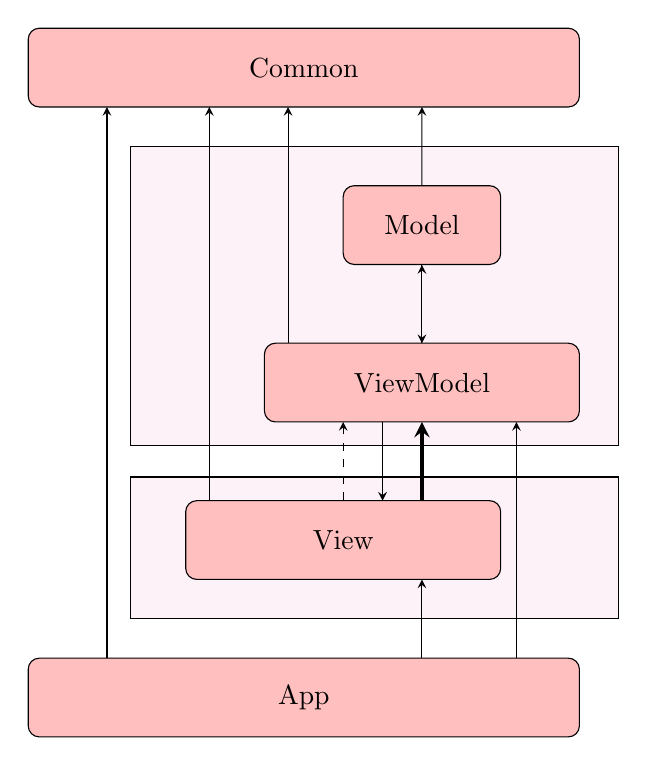
\begin{tikzpicture}
%define

\tikzstyle{state_s} = [rectangle, rounded corners, minimum width=2cm, minimum height=1cm, text centered, draw=black, fill = pink]
\tikzstyle{state_m} = [rectangle, rounded corners, minimum width=4cm, minimum height=1cm, text centered, draw=black, fill = pink]
\tikzstyle{state_l} = [rectangle, rounded corners, minimum width=7cm, minimum height=1cm, text centered, draw=black, fill = pink]
\tikzstyle{state_xl} = [rectangle, rounded corners, minimum width=7cm, minimum height=1cm, text centered, draw=black, fill = pink]
\tikzstyle{arrow} = [->, >=stealth]
\tikzstyle{arrowb} = [->, >=stealth, line width = 0.05cm]
\tikzstyle{arrowx} = [->, >=stealth, dashed]

%block1
\filldraw[fill = magenta, opacity = 0.05, draw opacity = 1](-2.2,-1)rectangle(4,-4.8);
%block2
\filldraw[fill = magenta, opacity = 0.05, draw opacity = 1](-2.2,-5.2)rectangle(4,-7);

\node[state_l, draw, align=left](state_Common){Common};
\node[state_s, below of = state_Common, xshift = 1.5cm, yshift = -1cm, draw, align=left](state_Model){Model};
\node[state_m, below of = state_Common, xshift = 1.5cm, yshift = -3cm, draw, align=left](state_VM){ViewModel};
\node[state_m, below of = state_Common, xshift = 0.5cm, yshift = -5cm, draw, align=left](state_View){View};
\node[state_xl, below of = state_Common, xshift = 0cm, yshift = -7cm, draw, align=left](state_App){App};
%line

\draw[arrow](state_Model)--(1.5,-0.5); %Model->Common
\draw[arrow](-0.2,-3.5)--(-0.2,-0.5); %ViewModel->Common
\draw[arrow](-1.2,-5.5)--(-1.2,-0.5); %View->Common
\draw[arrow](-2.5,-7.5)--(-2.5,-0.5); %App->Common
\draw[arrow](1.5,-2.5)--(1.5,-3.5); %Model->ViewModel
\draw[arrow](state_VM)--(state_Model);
\draw[arrowx](0.5,-5.5)--(0.5,-4.5); %View->ViewModel
\draw[arrow](1,-4.5)--(1,-5.5); %ViewModel->View
\draw[arrowb](1.5,-5.5)--(1.5,-4.5); %View->ViewModel(blue)
\draw[arrow](1.5,-7.5)--(1.5,-6.5); %App->View
\draw[arrow](2.7,-7.5)--(2.7,-4.5); %App->ViewModel

\end{tikzpicture}
\end{document}